\hypertarget{matrixmap_8h}{
\section{matrixmap.h File Reference}
\label{matrixmap_8h}\index{matrixmap.h@{matrixmap.h}}
}
{\tt \#include \char`\"{}matdata.h\char`\"{}}\par
{\tt \#include \char`\"{}matrices.h\char`\"{}}\par


Include dependency graph for matrixmap.h:\begin{figure}[H]
\begin{center}
\leavevmode
\includegraphics[width=104pt]{matrixmap_8h__incl}
\end{center}
\end{figure}


This graph shows which files directly or indirectly include this file:\begin{figure}[H]
\begin{center}
\leavevmode
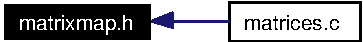
\includegraphics[width=104pt]{matrixmap_8h__dep__incl}
\end{center}
\end{figure}
\subsection*{Variables}
\begin{CompactItemize}
\item 
\begin{tabbing}
xx\=xx\=xx\=xx\=xx\=xx\=xx\=xx\=xx\=\kill
struct \{\\
\>char $\ast$ \hyperlink{matrixmap_8h_a0}{name}\\
\>const int($\ast$ \hyperlink{matrixmap_8h_a1}{mat} )\mbox{[}MATRIX\_SIZE\mbox{]}\\
\} \hyperlink{matrixmap_8h_a2}{matrix\_map} \mbox{[}$\,$\mbox{]}\\

\end{tabbing}\end{CompactItemize}


\subsection*{Detailed Description}
This file contains structures and functions for handling scoring matrices.

Definition in file \hyperlink{matrixmap_8h-source}{matrixmap.h}.

\subsection*{Variable Documentation}
\hypertarget{matrixmap_8h_a1}{
\index{matrixmap.h@{matrixmap.h}!mat@{mat}}
\index{mat@{mat}!matrixmap.h@{matrixmap.h}}
\subsubsection[mat]{\setlength{\rightskip}{0pt plus 5cm}const int($\ast$ \hyperlink{matrixmap_8h_a1}{mat})\mbox{[}MATRIX\_\-SIZE\mbox{]}}}
\label{matrixmap_8h_a1}




Definition at line 15 of file matrixmap.h.

Referenced by align\-Mat(), align\-Words\-Mat\_\-bit(), and main().\hypertarget{matrixmap_8h_a2}{
\index{matrixmap.h@{matrixmap.h}!matrix_map@{matrix\_\-map}}
\index{matrix_map@{matrix\_\-map}!matrixmap.h@{matrixmap.h}}
\subsubsection[matrix\_\-map]{\setlength{\rightskip}{0pt plus 5cm}struct \{ ... \}   \hyperlink{matrixmap_8h_a2}{matrix\_\-map}\mbox{[}$\,$\mbox{]}}}
\label{matrixmap_8h_a2}


This data structure maps the names of common matrices to the names of their variables

Referenced by get\-Matrix\-By\-Name().\hypertarget{matrixmap_8h_a0}{
\index{matrixmap.h@{matrixmap.h}!name@{name}}
\index{name@{name}!matrixmap.h@{matrixmap.h}}
\subsubsection[name]{\setlength{\rightskip}{0pt plus 5cm}char$\ast$ \hyperlink{matrixmap_8h_a0}{name}}}
\label{matrixmap_8h_a0}




Definition at line 14 of file matrixmap.h.
